\section{Definizione delle Variabili Linguistiche e delle Membership Functions}

Nel modello sono state introdotte quattro variabili linguistiche: tre in \emph{input} e una in \emph{output}.
\\\\
Di seguito sono presentate le 3 variabili di \emph{input}.

\subsection{Weather Condition}
La variabile \texttt{weather\_condition} rappresenta lo stato meteorologico e assume valori normalizzati nell'intervallo \([0,1]\), 
dove \(0\) corrisponde a condizioni pessime (\texttt{bad}) e \(1\) a condizioni ottimali (\texttt{good}).  

\begin{itemize}
  \item \textbf{Termini linguistici}:
    \begin{itemize}
      \item \texttt{bad}: trapezoidale definita dai punti [0.0, 0.0, 0.35, 0.65].
      \item \texttt{good}: trapezoidale definita dai punti  [0.35, 0.65, 1.0, 1.0].
    \end{itemize}
  \item \textbf{Universo}: \([0,1]\)
\end{itemize}

\noindent La Figura~\ref{Fig:mf_weather_condition} mostra le Membership Functions associate ai termini \texttt{bad} e \texttt{good}.

\begin{figure}[H]
    \centering
    \adjustbox{center}{
      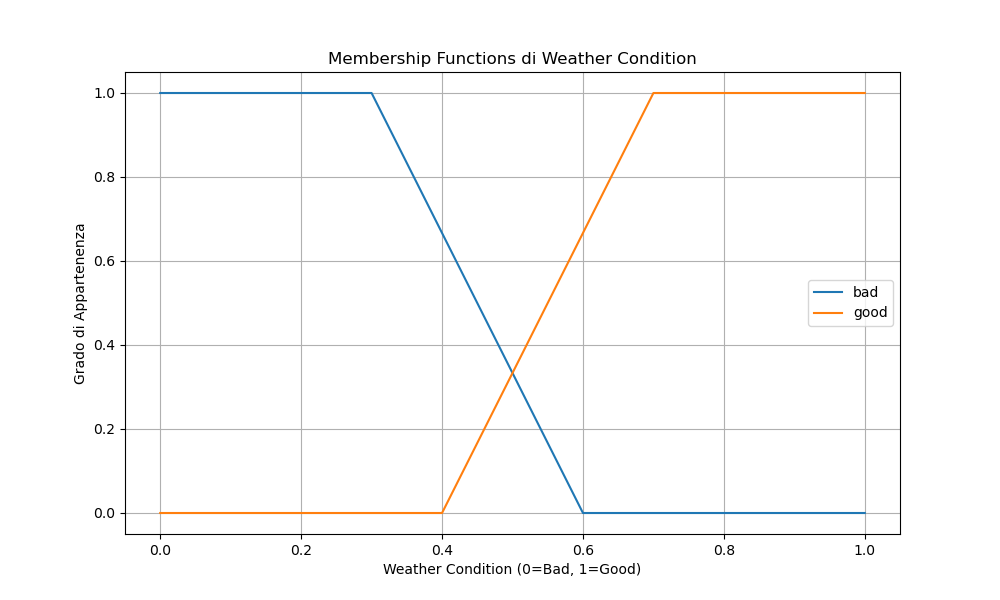
\includegraphics[width=1.2\linewidth]{membership_fun/weather_condition.png}
    }
    \caption{Membership Functions di Weather Condition.}
    \label{Fig:mf_weather_condition}
\end{figure}

\subsection{Time Headway}
La variabile \texttt{time\_headway} rappresenta il tempo necessario affinché il veicolo \emph{ego} 
percorra la distanza che lo separa dal veicolo \emph{leader}. È definita come:
\[
\text{time\_headway} \; [\mathrm{s}]
= \frac{\text{space\_gap}\;[\mathrm{m}]}{\text{ego\_velocity}\;[\mathrm{m}/\mathrm{s}]}
\]
dove \(\text{space\_gap}\) è la distanza tra i due veicoli ed \texttt{ego\_velocity} è la velocità del veicolo \emph{ego}. 
\paragraph{Annotazione} Si osservi che la formula impiega l'assunzione semplificativa 
secondo cui il veicolo \emph{leader} sia in grado di arrestarsi istantaneamente. 
Tale ipotesi, evidentemente irrealistica, trascura lo spazio di frenata necessario al \emph{leader}, 
che contribuirebbe ad aumentare il valore effettivo del \texttt{time\_headway}. Questa approssimazione 
è tuttavia considerata accettabile nell'ottica di una modellazione semplificata e risulta coerente con quanto 
previsto dalla normativa ACC ISO 15622:2018 \cite{iso15622}.

\begin{itemize}
  \item \textbf{Termini linguistici}:
    \begin{itemize}
      \item \texttt{dangerous}: trapezoidale definita dai punti [0.0, 0.0, 0.8, 1.5].
      \item \texttt{short}: triangolare definita dai punti [1.0, 2.0, 3.0].
      \item \texttt{adequate}: triangolare definita dai punti [2.5, 3.75, 5.0].
      \item \texttt{long}: triangolare definita dai punti [4.5, 5.75, 7.0].
      \item \texttt{very\_long}: trapezoidale definita dai punti [6.5, 7.0, 15.5, 15.5].
    \end{itemize}
  \item \textbf{Universo}: \([0,15.5]\) $\mathrm{s}$.  
        Il valore minimo corrisponde al limite fisico teorico, sebbene sia considerato praticamente irraggiungibile.
        Il valore massimo è stato determinato sulla base della portata tipica di un front radar sensor prodotto da BOSCH~\cite{bosch_radar}, pari a \(300\,\mathrm{m}\), e di una velocità minima del veicolo \emph{ego} pari a \(70\,\mathrm{km/h}\).  
        Pertanto, il massimo \texttt{time\_headway} è calcolato come:
        \[
            \max(\text{time\_headway})\,[\mathrm{s}] =
            \frac{300 \,[\mathrm{m}]}{\frac{70\,[\mathrm{km}/\mathrm{h}]}{3.6}} = 
            \frac{300 \,[\mathrm{m}]}{19.\overline{4}\,[\mathrm{m}/\mathrm{s}]}
            \approx 15.4\,[\mathrm{s}]
        \]
\end{itemize}

\begin{figure}[H]
    \centering
    \adjustbox{center}{
      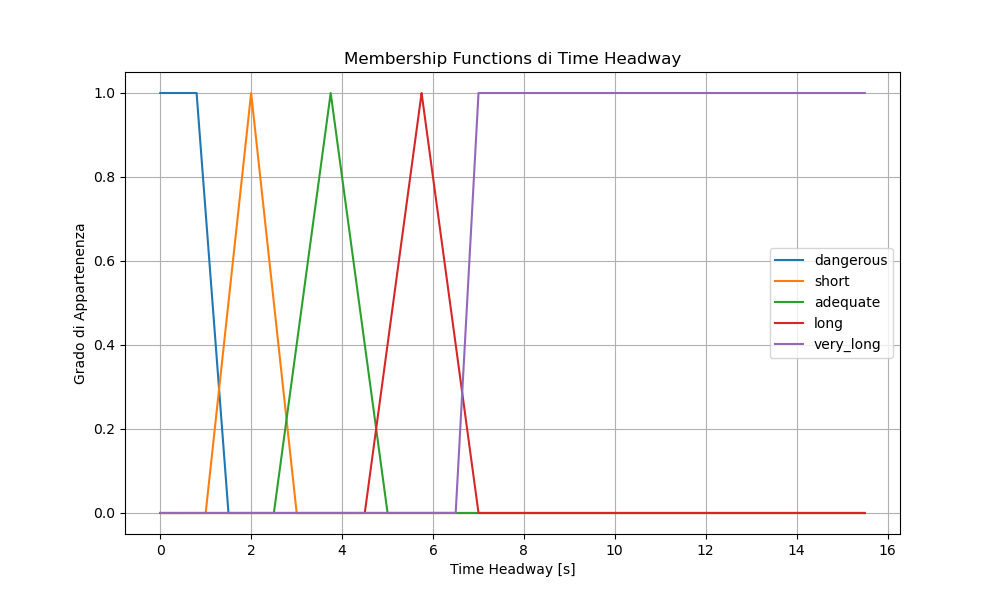
\includegraphics[width=1.2\linewidth]{membership_fun/time_headway.png}
    }
    \caption{Membership Functions di Time Headway}
    \label{Fig:mf_time_headway}
\end{figure}

\subsubsection{Motivazioni della Scelta della Variabile} 
\label{subsubsection:th_motivazione}
Si è preferito utilizzare la variabile \texttt{time\_headway} piuttosto che introdurre un insieme separato di variabili come 
\texttt{distanza}, \texttt{ego\_velocity} e \texttt{leader\_velocity}, sia per contenere la complessità del sistema riducendo 
il numero di regole da definire, sia perché le Membership Functions nei sistemi fuzzy non sono progettate per adattarsi 
dinamicamente in base a uno o più parametri.
\\\\
Ad esempio, risulterebbe problematico definire in modo univoco cosa significhi una distanza \texttt{dangerous}: quale intervallo 
tra \(0\,\mathrm{m}\) e \(300\,\mathrm{m}\) dovrebbe essere considerato tale? La pericolosità della distanza è infatti fortemente 
dipendente dalla velocità del veicolo.
\\\\
Consideriamo la relazione:
\begin{equation}
  d_{\mathrm{sicurezza}}\,[\mathrm{m}] = d_{\mathrm{reazione}}\,[\mathrm{m}] + d_{\mathrm{frenata}}\,[\mathrm{m}]
  \label{eq:d_sicurezza}
\end{equation}
\noindent dove \(d_{\mathrm{sicurezza}}\) rappresenta la distanza di sicurezza, \(d_{\mathrm{reazione}}\) è lo spazio percorso durante il tempo di reazione (ovvero il tempo necessario affinché il conducente inizi la frenata), e \(d_{\mathrm{frenata}}\) è lo spazio di arresto effettivo.
\\\\
Si ha:
\[
d_{\mathrm{reazione}} = v \cdot t
\]
dove \(v\) è la velocità del veicolo in \(\mathrm{m/s}\) e \(t\) è il tempo di reazione in secondi.
\\\\
Lo spazio di frenata è invece espresso da:
\[
d_{\mathrm{frenata}} = \frac{v^2}{2\,a\,\mu}
\]
dove \(a\) è la decelerazione massima e \(\mu\) è il coefficiente di attrito con il manto stradale (in condizioni ottimali pari a 0.8)~\cite{distanza_di_sicurezza_youmath}.
\\\\
Se due veicoli sono separati da \(20\,\mathrm{m}\), tale distanza risulta adeguata se la velocità 
dell'\emph{ego} è pari a \(30\,\mathrm{km/h}\). In tal caso, assumendo un tempo di reazione di \(1\,\mathrm{s}\), 
un coefficiente di attrito \(\mu=0.8\) e una brusca decelerazione pari a \(1\,g\) (ossia \(a = -9.81\,\mathrm{m/s^2}\)), si ottiene:
\[
d_{\mathrm{sicurezza}} = v \cdot t + \frac{v^2}{2\,a\,\mu}
\]
\[
d_{\mathrm{sicurezza}} 
= \frac{30 \,\left[{\frac{\mathrm{km}}{\mathrm{h}}}\right]}{3.6} \times 1\,\mathrm{[s]} 
+ \frac{\left(\frac{30 \,\left[{\frac{\mathrm{km}}{\mathrm{h}}}\right]}{3.6}\right)^2}{2 \times 9.81\,\mathrm{\left[ \tfrac{m}{s^2} \right]} \times 0.8} =
\]

\[
= 8.\overline{33}\,\mathrm{[m]} 
+ \frac{(8.\overline{33}\,\mathrm{\left[\tfrac{m}{s}\right]})^2}{15.7\,\mathrm{\left[\tfrac{m}{s^2}\right]}}
= 8.\overline{33}\,\mathrm{m} + \frac{69.4\,\left[{\frac{\mathrm{m^2}}{\mathrm{s^2}}}\right]}{15.7\,\left[{\frac{\mathrm{m}}{\mathrm{s^2}}}\right]} =
\]

\[
= 8.\overline{33}\,\mathrm{[m]} + 4.42\,\mathrm{[m]} 
\approx 12.75\,\mathrm{[m]}.
\]

\noindent Viceversa, alla velocità di \(130\,\mathrm{km/h}\), la medesima distanza di \(20\,\mathrm{m}\) risulterebbe del tutto insufficiente. 
Ricalcolando infatti la distanza di sicurezza da mantenere nelle stesse condizioni si ottiene:

\[
d_{\mathrm{sicurezza}} \approx 119.1\,\mathrm{[m]}
\]

\noindent La variabile \texttt{time\_headway} consente di modellare direttamente il tempo che separa i due veicoli 
indipendentemente dalla loro velocità assoluta o dalla distanza in metri. Di fatto, agisce come una forma di 
\emph{normalizzazione} del concetto di distanza, rendendolo più interpretabile e stabile all'interno del sistema fuzzy.

\subsubsection{Scelta degli intervalli} 
Per definire gli intervalli della variabile linguistica \texttt{time\_headway}, 
ci si è basati sulla cosiddetta \emph{regola dei 3 secondi}~\cite{benzinazero2016}, 
un criterio ampiamente adottato nella sicurezza stradale per garantire una distanza adeguata dal veicolo che precede. 
Tale regola stabilisce che, indipendentemente dalla velocità, il conducente dovrebbe mantenere almeno tre secondi di distanza 
temporale dal veicolo antistante, assicurando così il tempo necessario per reagire in caso di frenata improvvisa. 
\\\\
\noindent Partendo da questo principio, è stato definito l'intervallo per la categoria \texttt{adequate}. 
Successivamente, sono stati impostati gli intervalli per le categorie \texttt{dangerous} e \texttt{short}, 
seguiti da quelli per \texttt{long} e \texttt{very\_long}. 
\\\\
\noindent Per verificare la correttezza degli intervalli scelti, la Tabella \ref{tab:d_sicurezza_mantenuta} 
confronta la distanza da mantenere calcolata tramite l'equazione \ref{eq:d_sicurezza} con la distanza effettivamente mantenuta 
per i diversi valori di \texttt{ego\_velocity} e \texttt{time\_headway}. 
Nella tabella è inoltre riportata la differenza percentuale tra le due misure. 
\\\\
\noindent Si sottolinea che, per il calcolo di entrambe le distanze, sono stati utilizzati i valori $a = 9.81~\mathrm{m/s^2}$ 
e $\mu = 0.8$ come in precedenza, modificando però il tempo di reazione da $1~\mathrm{secondo}$ a $2~\mathrm{secondi}$, 
in quanto si presuppone che, in autostrada con ACC attivo, il conducente presti un livello di attenzione ridotto e impieghi
più tempo a reagire.

\begin{table}[h!]
\centering
\resizebox{\textwidth}{!}{
\begin{tabular}{|c|c|c|c|c|}
\hline
\textbf{\makecell{Velocità \\ {[}km/h{]}}} &
\textbf{\makecell{Time\\Headway [s]}} & 
\textbf{\makecell{Distanza da\\mantenere [m]}} & 
\textbf{\makecell{Distanza\\mantenuta [m]}} & 
\textbf{\makecell{Differenza \%}} \\
\hline
\multirow{8}{*}{70} & 0.5 & \multirow{8}{*}{62.977} & 33.810 & \textcolor{red}{-46.313} \\
                     & 1.0 &  & 43.533 & \textcolor{red}{-30.875}  \\
                     & 2.0 &  & 62.977 & 0.000  \\
                     & 3.0 &  & 82.421 & \textcolor[rgb]{0.0,0.5,0.0}{+30.875}    \\
                     & 4.0 &  & 101.866 & \textcolor[rgb]{0.0,0.5,0.0}{+61.751}  \\
                     & 7.0 &  & 160.199 & \textcolor[rgb]{0.0,0.5,0.0}{+154.377}  \\
                     & 10.0 &  & 218.533 & \textcolor[rgb]{0.0,0.5,0.0}{+247.004} \\
                     & 15.0 &  & 315.755 & \textcolor[rgb]{0.0,0.5,0.0}{+401.381} \\
\hline
\multirow{8}{*}{110} & 0.5 & \multirow{8}{*}{120.594} & 74.761 & \textcolor{red}{-38.006} \\
                     & 1.0 &  & 90.038 & \textcolor{red}{-25.338}  \\
                     & 2.0 &  & 120.594 & 0.000 \\
                     & 3.0 &  & 151.149 & \textcolor[rgb]{0.0,0.5,0.0}{+25.338}   \\
                     & 4.0 &  & 181.705 & \textcolor[rgb]{0.0,0.5,0.0}{+50.675}  \\
                     & 7.0 &  & 273.372 & \textcolor[rgb]{0.0,0.5,0.0}{+126.688}  \\
                     & 10.0 &  & 365.038 & \textcolor[rgb]{0.0,0.5,0.0}{+202.700} \\
                     & 15.0 &  & 517.816 & \textcolor[rgb]{0.0,0.5,0.0}{+329.388} \\
\hline
\multirow{8}{*}{150} & 0.5 & \multirow{8}{*}{193.942} & 131.442 & \textcolor{red}{-32.226} \\
                     & 1.0 &  & 152.275 & \textcolor{red}{-21.484} \\
                     & 2.0 &  & 193.942 & 0.000 \\
                     & 3.0 &  & 235.609 & \textcolor[rgb]{0.0,0.5,0.0}{+21.484}   \\
                     & 4.0 &  & 277.275 & \textcolor[rgb]{0.0,0.5,0.0}{+42.968}  \\
                     & 7.0 &  & 402.275 & \textcolor[rgb]{0.0,0.5,0.0}{+107.421}  \\
                     & 10.0 &  & 527.275 & \textcolor[rgb]{0.0,0.5,0.0}{+171.873} \\
                     & 15.0 &  & 735.609 & \textcolor[rgb]{0.0,0.5,0.0}{+279.293} \\
\hline
\end{tabular}
}
\caption{Confronto tra distanza di sicurezza da mantenere e distanza mantenuta.}
\label{tab:d_sicurezza_mantenuta}
\end{table}

\subsection{Relative Velocity}
La variabile \texttt{relative\_velocity} rappresenta la velocità relativa del veicolo \emph{leader} rispetto al veicolo \emph{ego}.
Essa è definita come:
\[
\text{relative\_velocity}\,\left[\frac{\mathrm{m}}{\mathrm{s}}\right] = \text{leader\_velocity}\,\left[\frac{\mathrm{m}}{\mathrm{s}}\right] - \text{ego\_velocity}\,\left[\frac{\mathrm{m}}{\mathrm{s}}\right].
\]
\paragraph{Annotazione} Si noti che, sebbene la variabile rappresenti la velocità relativa del \emph{leader} rispetto all'\emph{ego}, 
i termini linguistici sono definiti dal punto di vista dell'\emph{ego}. Ad esempio, se il \emph{leader} viaggia a $30\,\frac{\mathrm{m}}{\mathrm{s}}$ e 
l'\emph{ego} a $20\,\frac{\mathrm{m}}{\mathrm{s}}$, si ha:
\[
\text{relative\_velocity} = 10\,\left[\frac{\mathrm{m}}{\mathrm{s}}\right],
\]
ossia il \emph{leader} è $36\,\frac{\mathrm{km}}{\mathrm{h}}$ più veloce dell'\emph{ego}. In questo caso, il fenomeno rientra nella categoria 
\texttt{moving\_away\_fast}, poiché l'\emph{ego} si sta allontanando rapidamente dal leader.
\begin{itemize}
  \item \textbf{Termini linguistici}:
    \begin{itemize}
      \item \texttt{approaching\_fast}: trapezoidale definita dai punti [-23.0, -23.0, \\ -10.0, -5.0].
      \item \texttt{approaching}: triangolare definita dai punti [-7.0, -3.0, -0.5].
      \item \texttt{steady}: triangolare definita dai punti [-1.0, 0.0, 1.0].
      \item \texttt{moving\_away}: triangolare definita dai punti [0.5, 3.0, 7.0].
      \item \texttt{moving\_away\_fast}: trapezoidale definita dai punti [5.0, 10.0, 23.0, 23.0].
    \end{itemize}
  \item \textbf{Universo}: \([-23.0,+23.0]\) $\frac{\mathrm{m}}{\mathrm{s}}$
\end{itemize}
Gli estremi dell'universo sono stati determinati calcolando, in valore assoluto, la massima differenza di velocità tra il veicolo
\emph{leader} e il veicolo \emph{ego}, come mostrato di seguito:
\[
  \max(\text{relative\_velocity}) \,\left[\frac{\mathrm{m}}{\mathrm{s}}\right]
  = \frac{150\,\left[\frac{\mathrm{km}}{\mathrm{h}}\right] - 70\,\left[\frac{\mathrm{km}}{\mathrm{h}}\right]}{3.6}
  = 22.\overline{2}\,\left[\frac{\mathrm{m}}{\mathrm{s}}\right]
\]

\noindent In Figura~\ref{Fig:mf_relative_velocity} sono riportate le Membership Functions associate alla variabile \texttt{relative\_velocity}.
\begin{figure}[H]
    \centering
    \adjustbox{center}{
      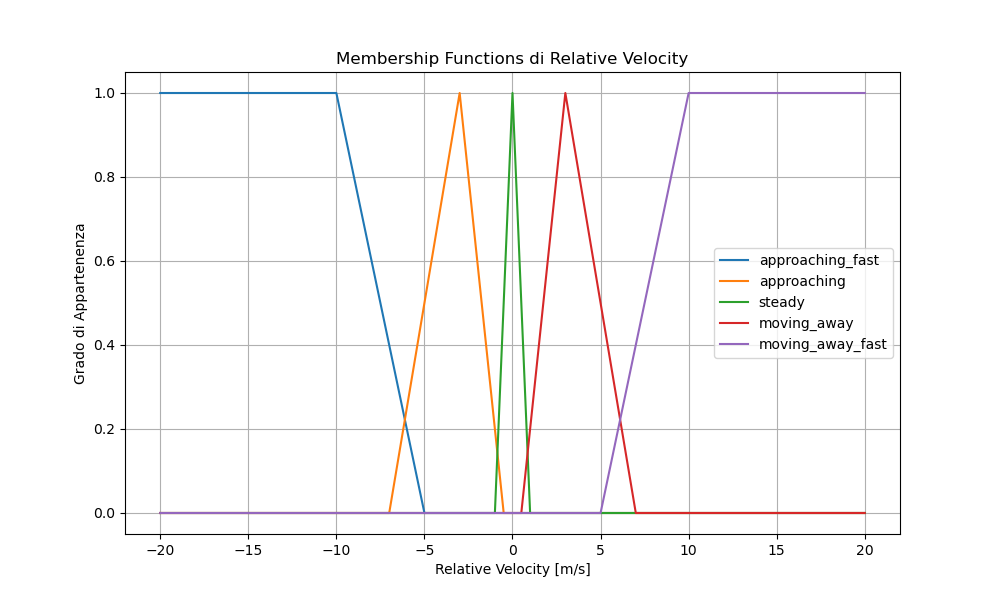
\includegraphics[width=1.2\linewidth]{membership_fun/relative_velocity.png}
    }
    \caption{Membership Functions di Relative Velocity}
    \label{Fig:mf_relative_velocity}
\end{figure}

\vspace{10mm}
\noindent Di seguito viene presentata l'unica variabile in \emph{output}.

\subsection{Acceleration}
La variabile \texttt{acceleration} rappresenta l'accelerazione (positiva, negativa o nulla) impartita al veicolo:
\begin{itemize}
  \item \textbf{Termini linguistici}:
    \begin{itemize}
      \item \texttt{strong\_deceleration}: trapezoidale definita dai punti [-3.0, -3.0, \\ -2.5, -2.0].
      \item \texttt{medium\_deceleration}: triangolare definita dai punti [-2.5, -1.8, -1.0].
      \item \texttt{light\_deceleration}: triangolare definita dai punti [-1.2, -0.7, -0.2].
      \item \texttt{zero\_acceleration}: trapezoidale definita dai punti [-0.3, -0.1, 0.1, 0.3].
      \item \texttt{light\_acceleration}: triangolare definita dai punti [0.2, 0.7, 1.2].
      \item \texttt{medium\_acceleration}: triangolare definita dai punti [1.0, 1.8, 2.5].
      \item \texttt{strong\_acceleration}: trapezoidale definita dai punti [2.0, 2.5, 3.0, 3.0].
    \end{itemize}
    \noindent Si noti che per il termine \texttt{zero\_acceleration} è stata scelta una funzione \textbf{trapezoidale}, anziché triangolare.  
  Questa decisione consente di rappresentare un intervallo più ampio di valori prossimi allo zero come “assenza di accelerazione”, evitando che piccolissime variazioni (inevitabili nei sensori o nel modello) vengano interpretate come continue micro-accelerazioni o micro-decelerazioni.  
  In questo modo il sistema risulta più stabile e garantisce una guida percepita come più confortevole dal conducente.
  \item \textbf{Universo}: \([-3.0,+3.0]\)\,$\frac{\mathrm{m}}{\mathrm{s^2}}$
\end{itemize}
Un'accelerazione al di fuori di tale intervallo è considerata non confortevole e quindi incompatibile con l'obiettivo di comfort che il sistema ACC deve garantire.  
In particolare:
\begin{itemize}
  \item Una \textbf{decelerazione superiore in modulo a \(-3\,\tfrac{\mathrm{m}}{\mathrm{s^2}}\)} 
  è considerata troppo brusca, poiché va oltre il valore raccomandato 
  dall'\textit{Institute of Transportation Engineers} (ITE, 1999), pari a \(3.0\,\tfrac{\mathrm{m}}{\mathrm{s^2}}\) \cite{comfortable_deceleration_rate}; 
  in questi casi l'intervento viene demandato all'AEB (Autonomous Emergency Braking), un sistema ADAS distinto 
  incaricato della gestione delle frenate di emergenza.
  \item Un'accelerazione \textbf{superiore a \(+3\,\tfrac{\mathrm{m}}{\mathrm{s^2}}\)} è considerata eccessiva e non 
  confortevole per il conducente e i passeggeri.
\end{itemize}

\noindent In Figura~\ref{Fig:mf_acceleration} sono riportate le Membership Functions associate alla variabile \texttt{acceleration}.
\begin{figure}[H]
    \centering
    \adjustbox{center}{
      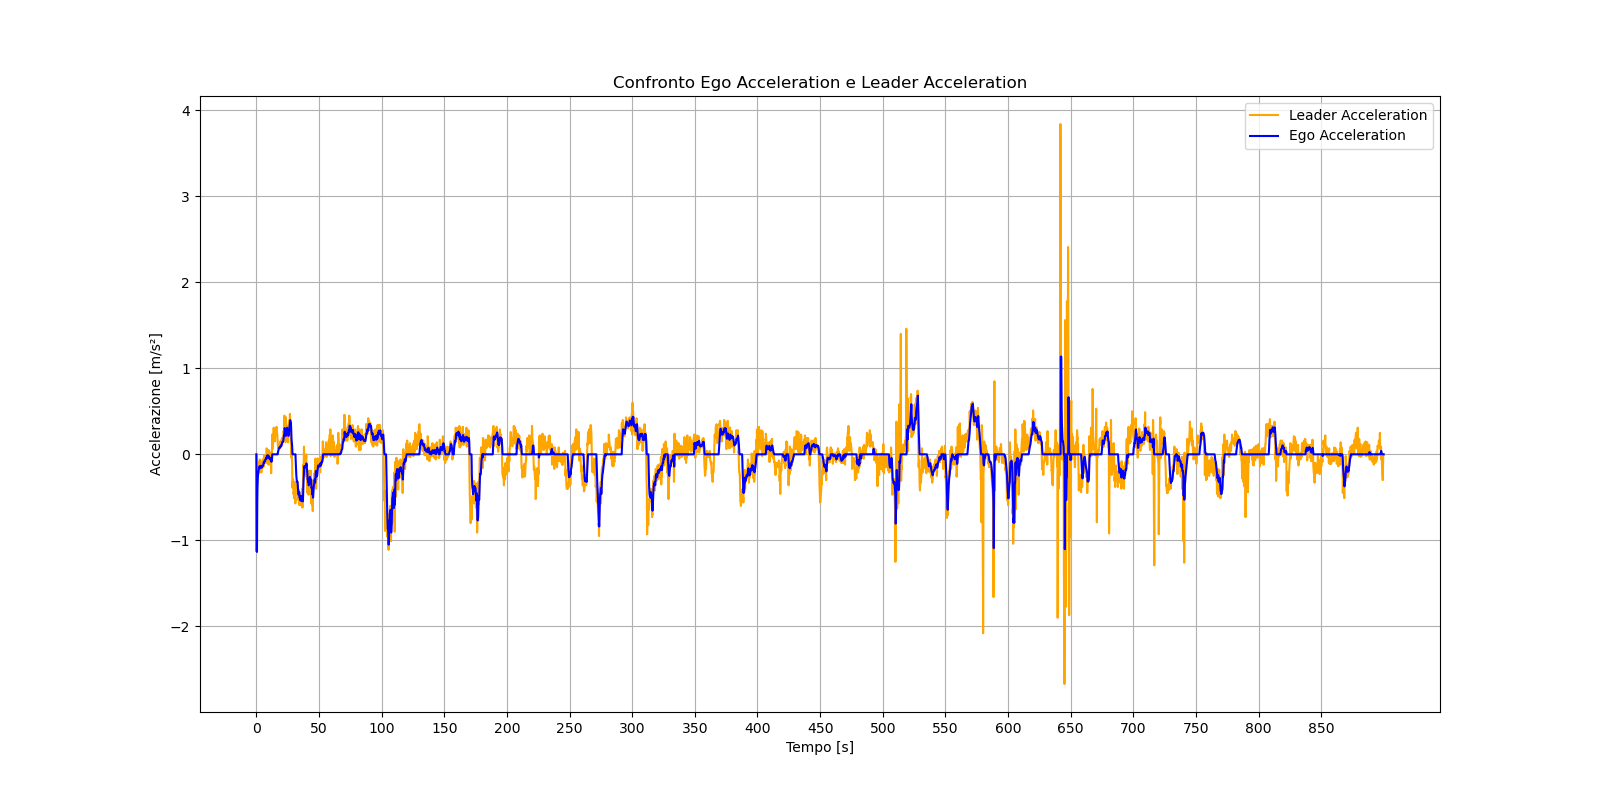
\includegraphics[width=1.1\textwidth]{membership_fun/acceleration.png}
    }  
    \caption{Membership Functions di Acceleration}
    \label{Fig:mf_acceleration}
\end{figure}